%!TEX root = Slic3r-Manual.tex

\subsection{Configuration Wizard}
\label{sec:configuration_wizard}
\index{Configuration Wizard}

Slic3r has two features to aid newcomers: the configuration wizard, and simple mode.

Sometimes it is nice to have a helping hand when starting out with new software.  The configuration wizard asks a series of questions and creates a configuration for Slic3r to start with.

\textbf{When using the pre-set TAZ Slic3r profiles you do not need to complete the Configuration Wizard.} The Configuration Wizard can be later accessed from the top menu once you are ready to start creating your own Slic3r profiles.

\begin{figure}[H]
\centering
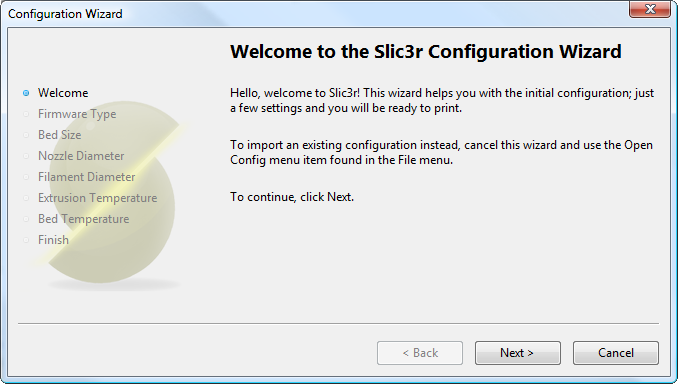
\includegraphics[keepaspectratio=true,width=\textwidth]{configuration_wizard/configuration_wizard_welcome.png}
\caption{Configuration Wizard: Welcome Screen}
\label{fig:configuration_wizard_welcome_screen}
\end{figure}

\newpage
\subsubsection{1. Firmware Type}
\label{sub:1_firmware_type}
\index{Printer Settings!Firmware!G-code flavour}
The gcode produced by Slic3r is tailored to particular types of firmware.  The first step prompts for the firmware that the printer uses.  For the TAZ printer select \texttt{RepRap (Marlin/Sprinter)}
\begin{figure}[H]
\centering
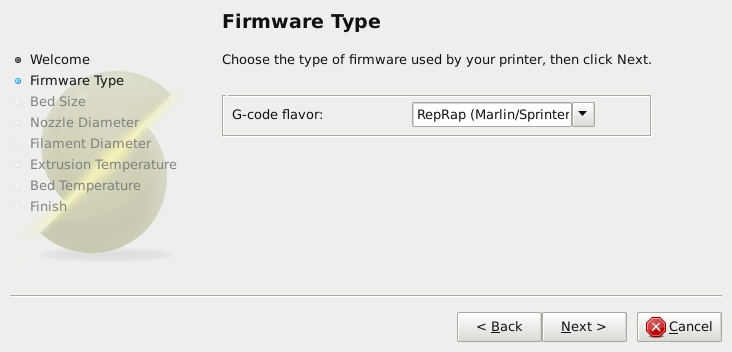
\includegraphics[keepaspectratio=true,width=\textwidth]{configuration_wizard/configuration_wizard_firmware_type.png}
\caption{Configuration Wizard: Firmware Type}
\label{fig:configuration_wizard_firmware_type}
\end{figure}

\newpage
\subsubsection{2. Bed Size}
\label{sub:2_bed_size}
\index{Printer Settings!Size and coordinates!Bed size}
This setting defines the maximum distance the extruder may travel along the X and Y axis.  The dimension for the TAZ print surface are X: 298 and Y: 280.

Be sure to measure from the lower left corner where the extruder nozzle rests when are the home position to the maximum distance the nozzle can travel in each direction.  Take into account that the X carriage may touch the frame before the nozzle reaches it's full distance, this will depend on the printer make and model.

\begin{figure}[H]
\centering
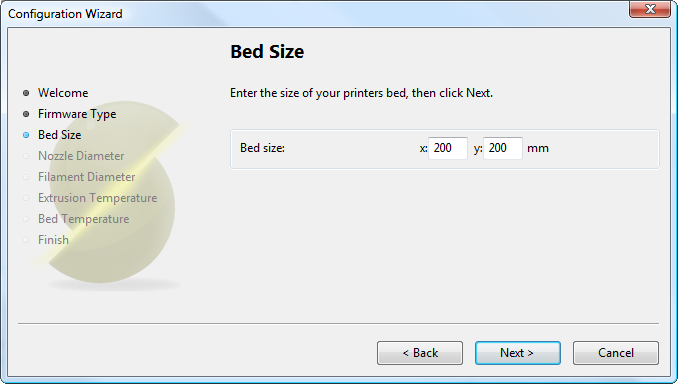
\includegraphics[keepaspectratio=true,width=\textwidth]{configuration_wizard/configuration_wizard_bed_size.png}
\caption{Configuration Wizard: Bed Size}
\label{fig:configuration_wizard_bed_size}
\end{figure}

\newpage
\subsubsection{3. Nozzle Diameter}
\label{sub:3_nozzle_diameter}
\index{Printer Settings!Extruder!Nozzle diameter}
The diameter of the hot-end nozzle is usually clearly displayed either in the description of the hot-end, or in the associated documentation, when the hot-end is purchased.  The default nozzle size on the TAZ hot end is 0.35mm.

If the nozzle was home-made, or came from a source without a diameter given, then carefully measure the aperture as accurately as possible.  One way of determining nozzle size is to very slowly (1mm/s) extrude some filament into free air and measure the thickness of the resulting extrusion\footnote{\	http://forums.reprap.org/read.php?1,113374,113953}.  This has the benefit of taking die swell into account, and consequently may be a useful thing to do even if the diameter is known.

\begin{figure}[H]
\centering
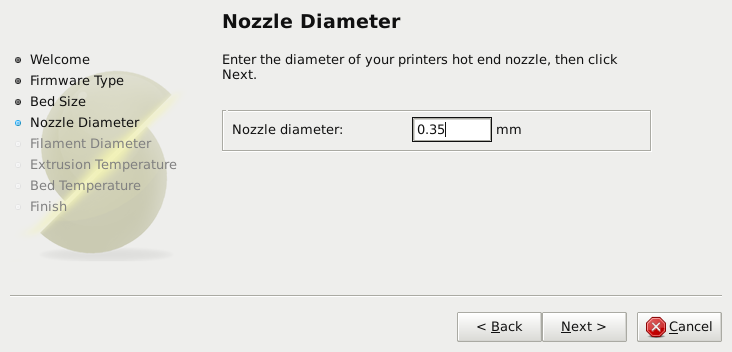
\includegraphics[keepaspectratio=true,width=\textwidth]{configuration_wizard/configuration_wizard_nozzle_diameter.png}
\caption{Configuration Wizard: Nozzle Diameter}
\label{fig:configuration_wizard_nozzle_diameter}
\end{figure}

\newpage
\subsubsection{4. Filament Diameter}
\label{sub:4_filament_diameter}
\index{Filament Settings!Filament!Diameter}
For Slic3r to produce accurate results it must know as accurately as possible how much material is pushed through the extruder.  Therefore it is vital to give it as precise a value as possible for the filament diameter.

Although the filament used in FDM printers is sold as being either 3mm or 1.75mm this is only a general guide.  The diameter can vary between manufacturers and even between batches.  Therefore it is highly recommended to take multiple measurements from along a length of the filament and use the average.  For example, measurements of 2.89, 2.88, 2.90 and 2.91 would yield an average of 2.895, and so this would be used.

\begin{figure}[H]
\centering
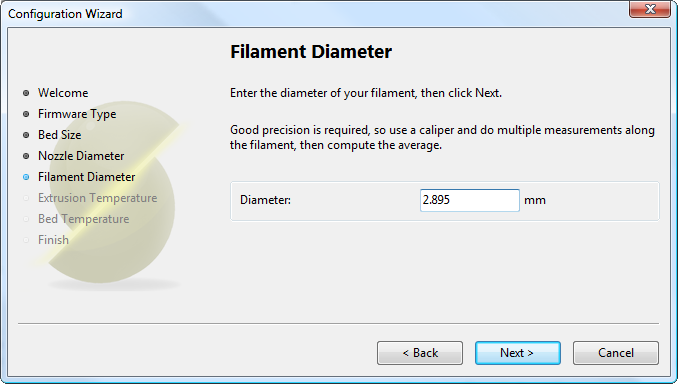
\includegraphics[keepaspectratio=true,width=\textwidth]{configuration_wizard/configuration_wizard_filament_diameter.png}
\caption{Configuration Wizard: Filament Diamter}
\label{fig:configuration_wizard_filament_diameter}
\end{figure}

\newpage
\subsubsection{5. Extrusion Temperature}
\label{sub:5_extrusion_temperature}
\index{Filament Settings!Temperature!Extruder}
The extrusion temperature will depend on the material, and most can operate over a range of temperatures.  The supplier should provide guidance as to which temperatures are suitable.  A very general rule of thumb is that PLA lies between 160°C and 230°C, and ABS lies between 220°C and 240°C. More exotic materials will have a different range.

This is one parameter which you will want to fine tune when you start producing prints.  The optimal temperature can vary even between colors of the same material.  Another factor which may affect the chosen temperature is how fast the extrusion is, where generally faster extrusion runs hotter.

\textbf{Note: One may choose to control the extruder temperature manually from the printer controller. In this case the temperature can be set to zero.}

\begin{figure}[H]
\centering
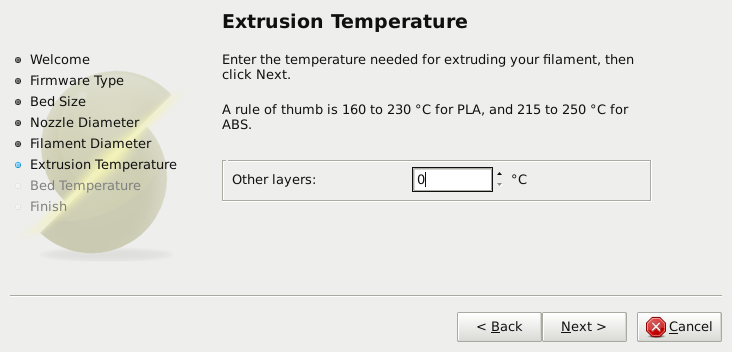
\includegraphics[keepaspectratio=true,width=\textwidth]{configuration_wizard/configuration_wizard_extrusion_temperature.png}
\caption{Configuration Wizard: Extrusion Temperature}
\label{fig:configuration_wizard_extrusion_temperature}
\end{figure}

\newpage
\subsubsection{6. Bed Temperature}
\label{sub:6_bed_temperature}
\index{Filament Settings!Temperature!Bed}
If the printer has a heated bed then this parameter may be set.  As with the extruder temperature, the value will depend on the material used.  A rule of thumb is that PLA requires 35°C - 60°C and ABS requires 85°C.

\textbf{Note: One may choose to control the bed temperature manually from the printer controller. In this case the temperature can be set to zero.}

\begin{figure}[H]
\centering
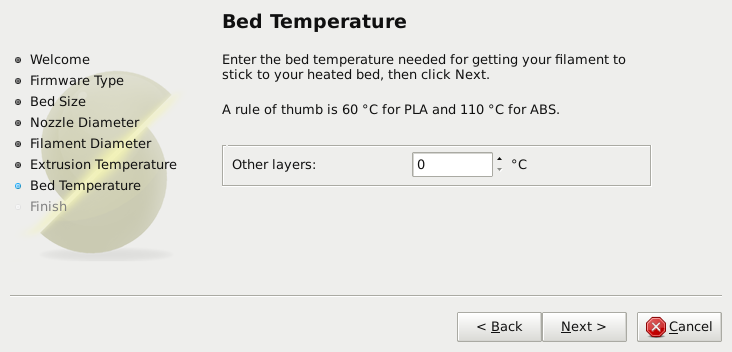
\includegraphics[keepaspectratio=true,width=\textwidth]{configuration_wizard/configuration_wizard_bed_temperature.png}
\caption{Configuration Wizard: Bed Temperature}
\label{fig:configuration_wizard_bed_temperature}
\end{figure}

\newpage

At this stage the wizard is complete and the basic configuration is defined.

\begin{figure}[H]
\centering
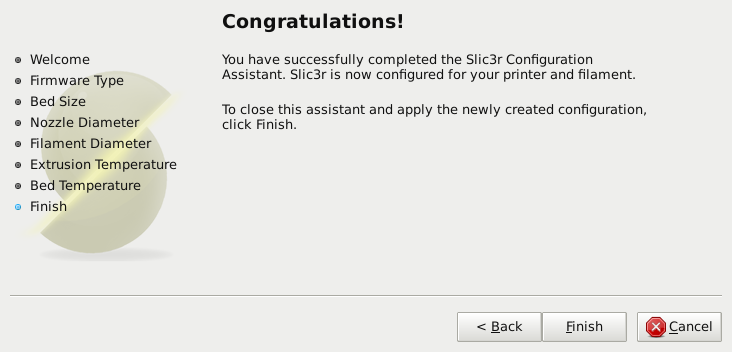
\includegraphics[keepaspectratio=true,width=\textwidth]{configuration_wizard/configuration_wizard_end.png}
\caption{Configuration Wizard: End}
\label{fig:configuration_wizard_end}
\end{figure}

